 \chapter{Introduction}

\section{Scope of the Problem}\label{problem}
In 2017, breast cancer in females was estimated to be the most common cancer in the whole of Australia, and the fourth highest cause of cancer-related deaths \cite{australian_institute_of_health_and_welfare_cancer_2017}, with Australian women having a 1 in 8 chance of being diagnosed before the age of 85 \cite{australian_institute_of_health_and_welfare_breast_2012}. However with the current abilities of breast cancer screening, Australia has one of the best breast cancer survival rates, at approximately 90\% \cite{australian_institute_of_health_and_welfare_breast_2012}, where the treatment is in most cases removal of the diseased breast tissue (lumpectomy) or removal of the entire breast (masectomy), often used alongside less target-specific radiotherapy. In both cases, it is of the utmost importance for the surgeon to remove all cancerous tissue from the patient, otherwise the patient is required to undergo the surgery procedure again (a re-excision) to remove the rest of the tumour. For patients that initially underwent breast-conserving surgery in the form of a lumpectomy, most prefer to undergo a full masectomy to minimize the risk of the cancer recurring, a decision that has great significance in terms of operation cost and the cosmetic outcome of the surgery, as well as cause significant patient anxiety.

\begin{figure}
	\centering
    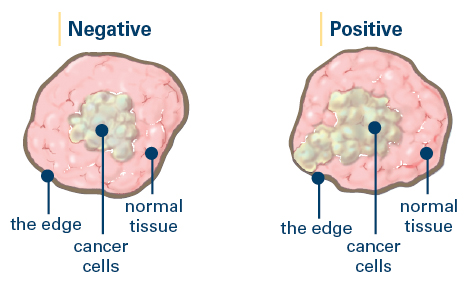
\includegraphics[width=0.6\textwidth]{figures/margins.png}
    \label{margins}
    \caption{Surgical margin assessment examples of a) negative and b) positive margins. Taken from \cite{breastcancer.org_surgical_2017}}
\end{figure}

A study in 2015 \cite{ballal_predictors_2015} found that in Western Australia, there was a re-excision rate of 30\% for wire-guided breast conserving surgery. It is recommended that a surgical margin of $2mm$ of healthy tissue be left around the excised tumour, to reduce the risk of future recurrence of cancer in the patient \cite{behm_surgical_2013}. The high re-excision rate is due to the inability of surgeons to determine whether an excised tissue has positive (cancerous tissue on the boundary) or negative (tumour-free, see autoref{margins}) margins during surgery, but only after it has been sent through pathology. Use of an imaging method capable of examining excised tissue boundaries (or even tissue boundaries within the breast cavity itself) with high specificity and sensitivity during surgery would likely decrease this re-excision rate \cite{ballal_predictors_2015}. The section below describes one possible imaging method that could be used to address this problem. 

\section{Elastography}\label{elastography}
Elastography uses the application of an external mechanical load on a tissue to produce images of mechanical contrast, such as stiffness (elasticity) of the tissue. The sense of touch used by a surgeon to differentiate stiff tumour from softer healthy tissue is analogous to elastography on a much coarser scale, however elastography has the potential to enable quantitative images of the mechanical properties of tissue to be formed on a much smaller scale. The use of optical imaging techniques as underlying imaging tools for elastography allow much higher resolution imaging, providing access to the mechanical properties of tissues on the micrometre scale \cite{schmitt_oct_1998} \cite{kennedy_review_2014}.
These maps of mechanical properties of tissue offer insight into the study of disease at scales varying from organs to tissue micro-architecture, which can be probed by utilising different imaging techniques to investigate the deformation of the tissue.

\section{The OCE Solution}\label{solution}
\begin{figure}
	\centering
    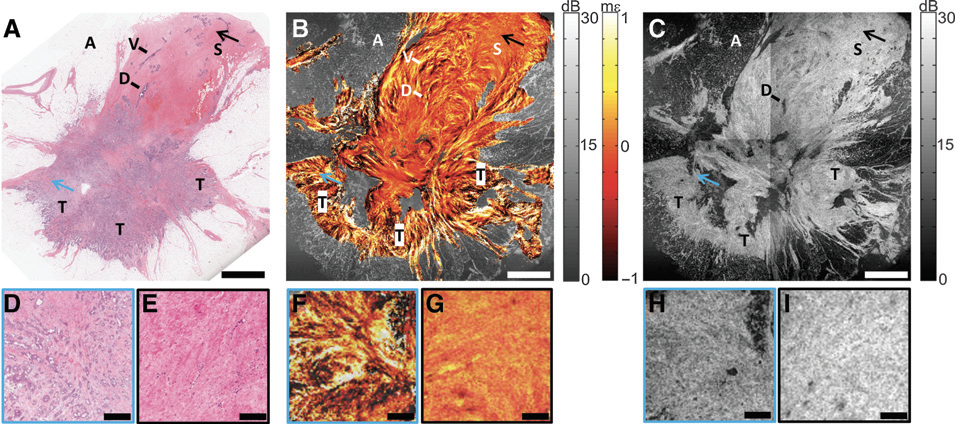
\includegraphics[width=\textwidth]{figures/oce_example.png}
    \label{oce_example}
    \caption{An example OCE image of breast tissue, taken from \cite{kennedy_investigation_2015}. The histology is shown on the far left, the strain elastogram image in the centre, and the OCT image on the right. Below the main images, regions of tumour (left) and healthy stroma (right) are presented side-by-side for contrast for each imaging technique.}
\end{figure}

Elastography techniques commonly used with optical imaging modalities, among others, can be thought of in three categories: compressive, resonant and shear wave based elastography. Static or quasi-static methods of loading include compressing the tissue, either through an indentation point or in bulk, and measures the resulting strain in the tissue by detecting the displacement vector produced between two image acquisitions \cite{kennedy_optical_2014}. This displacement can be used to calculate the local strain at different points in the image, to which elasticity is inversely related. Resonant loading methods, that impart a step load using acoustic radiation force or magnetomotive forces record the natural frequency of the tissue, whose square is directly proportional to elasticity \cite{kennedy_optical_2015}. Shear wave techniques use the phase velocity of a propagating wave within the tissue as a mechanical contrast parameter, as generated by a pulsed or periodic load. 

As outlined in \autoref{problem}, there is a clear need for intra-operative imaging tools capable of resolving small amounts of cancerous tissue at surgical margins in breast conserving surgery. Having a surgical tool capable of real-time in vivo imaging of excised tissue boundaries has the potential to reduce the re-excision rates in breast cancer patients.

Optical coherence elastography (OCE) utilises optical coherence tomography (OCT) as the underlying imaging technique, which relies on the optical properties of tissue to generate contrast in an image formed by backscattered light. An example of an OCE image is shown in \autoref{oce_example}, taken from \cite{kennedy_investigation_2015}. The significance of OCE lies in its ability to provide high resolution images at low sample depths. These properties differentiate it from other techniques, such as ultrasound elastography, which could be used to image deep within the body due to the higher penetration of sound waves into tissue. The ideal application of OCE is at surface tissue (such as imaging the retina, or skin), on excised tissue in a surgical setting, or used as a tool during surgery on uncovered tissue. The third application forms the main motive for this project.

To be able to provide real-time OCE images in surgery, the processing of the optical data from the OCT system to produce elastography images must be done in real-time also. One way to speed up the processing is to remove the need for quantitative analysis, and use qualitative only. That is, to focus on the detectable difference between healthy and cancerous tissue using qualitative images only. Standard OCE elastograms (elastography images), combine measurements of both strain and stress to produce quantitative maps of tissue elasticity. However, to produce qualitative images of tissue mechanical properties, that differentiate softer from stiffer objects (such as healthy stroma from tumour), requires only images of strain. 

\section{Project Aims}\label{aims}

The current strain estimation algorithms, such as those used by the Bio-imaging Research and Innovation for Translational Engineering (BRITELab) to process strain on a bench top OCE system, are capable of scanning a 3D volume in about (??). In order to process strain in real-time, this must be sped up by a factor of (??). The purpose of this thesis is to investigate techniques of speeding up the processing of strain in OCE, for the purpose of real-time surgical application in breast cancer surgery. The goal is to compare strain estimation techniques on a simulated phantom using metrics of processing time (as an indication of its ability to be extended to real-time surgical application) and sensitivity (to monitor image quality). Once the strain estimation technique has been narrowed down to a small selection of optimal methods, the resulting image resolution is investigated as a measure of the ability to detect object boundaries in strain elastograms. Maintaining high image quality with much faster processing techniques in OCE strain estimation brings the goal of applying OCE imaging to real-time, intra-operative assessment of breast cancer margins, and hopefully resulting in reduced re-excision rates for breast cancer patients. 


